\subsection{Variance}
\begin{lstlisting}[language={},numbers=left,numberstyle=\tiny,frame = single]
Variance for redshift is 0.010498
\end{lstlisting}
\subsection{Deep Network for Regression}
I have tested both the GradientDescentOptimizer and the AdamOptimizer, and saw that the AdamOptimizer is superior in performance. However, plots of both are available below.

Some of the lines I have changed were:

\begin{lstlisting}[language=python,numbers=left,numberstyle=\tiny,frame=single,breaklines=true,postbreak=\mbox{\textcolor{red}{$\hookrightarrow$}\space}]
#change the activation to ReLU
y_1 = tf.matmul(x_data , W_1 ) + b_1
y_1 = tf.nn.relu(y_1)
\end{lstlisting}

\begin{lstlisting}[language=python,numbers=left,numberstyle=\tiny,frame=single,breaklines=true,postbreak=\mbox{\textcolor{red}{$\hookrightarrow$}\space}]
#change the loss function to MSE
loss = tf.reduce_mean(tf.square(model_output - y_target), name='mean_squared_error')
\end{lstlisting}

\begin{lstlisting}[language=python,numbers=left,numberstyle=\tiny,frame=single,breaklines=true,postbreak=\mbox{\textcolor{red}{$\hookrightarrow$}\space}]
#change the optimizer to ADAM
# Declare optimizer
my_opt =  tf.train.AdamOptimizer(FLAGS.lr)
train_step = my_opt.minimize(loss)
\end{lstlisting}


\begin{lstlisting}[language={},numbers=left,numberstyle=\tiny,frame=single,breaklines=true,postbreak=\mbox{\textcolor{red}{$\hookrightarrow$}\space}]
Iteration: 30000 / 30000
final training accuracy: 0.000976738
final test accuracy:  0.00126395 
final validation accuracy:  0.0010332
INFO:tensorflow:Restoring parameters from tensor_logs/bestNetwork
best training accuracy: 0.000954459 
best test accuracy:  0.00125532 
best validation accuracy:  0.000915237
\end{lstlisting}


\subsection{TensorBoard}

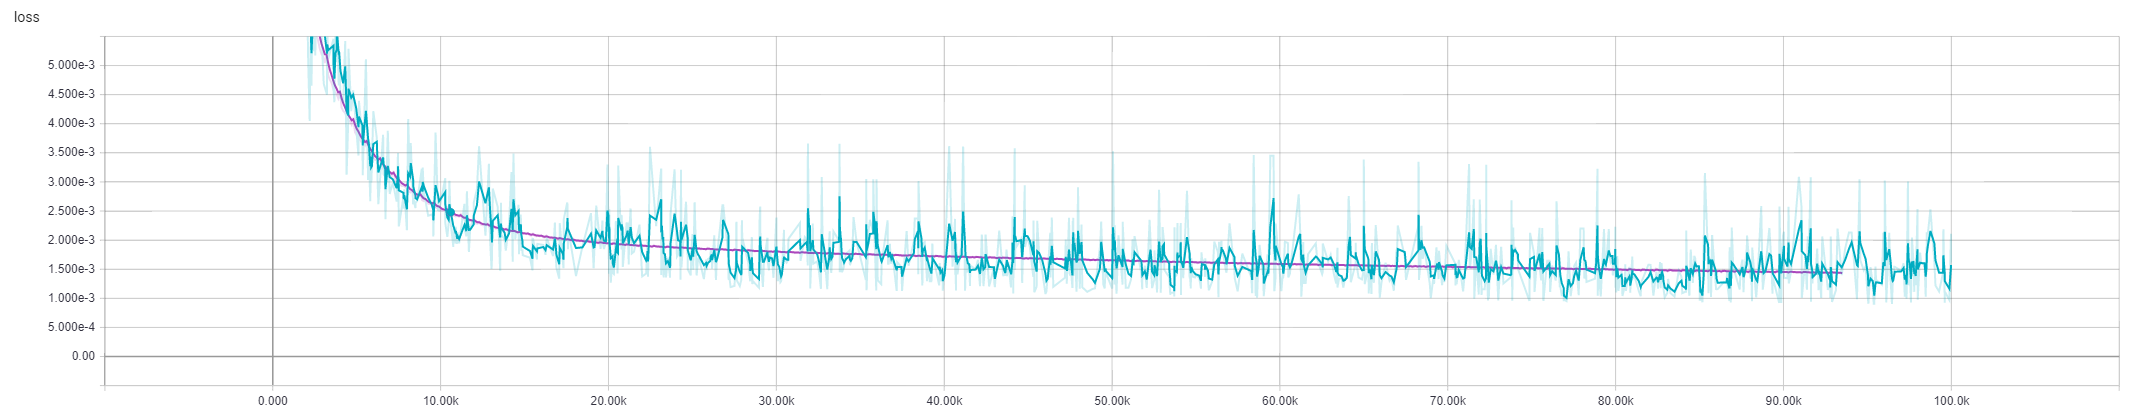
\includegraphics[width=15cm]{tf_relu_gradientdescent.png}

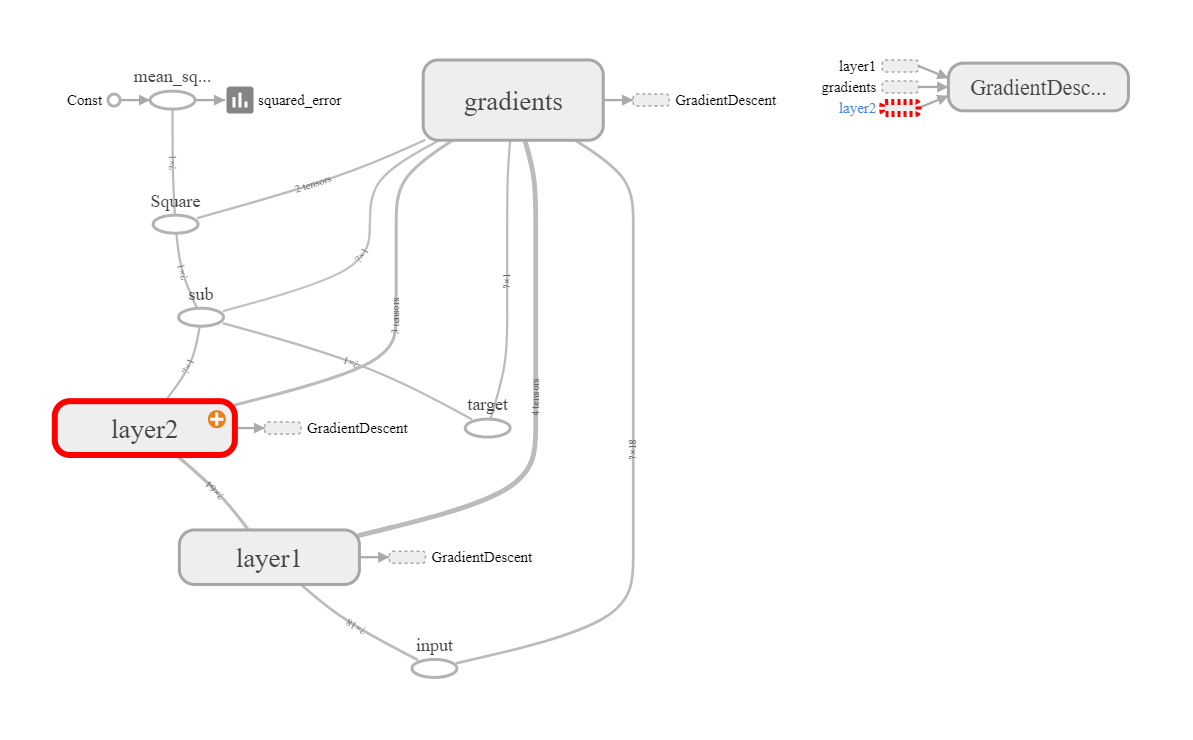
\includegraphics[width=13cm]{graph_relu_gradientdescent.png}

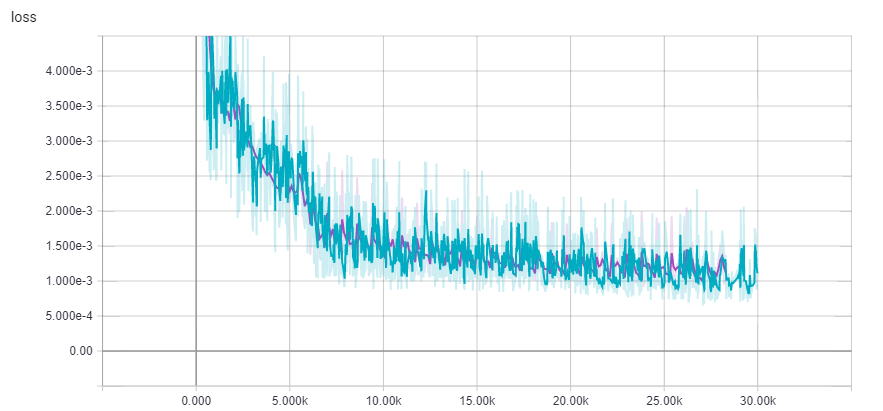
\includegraphics[width=15cm]{tf_relu_adam.png}

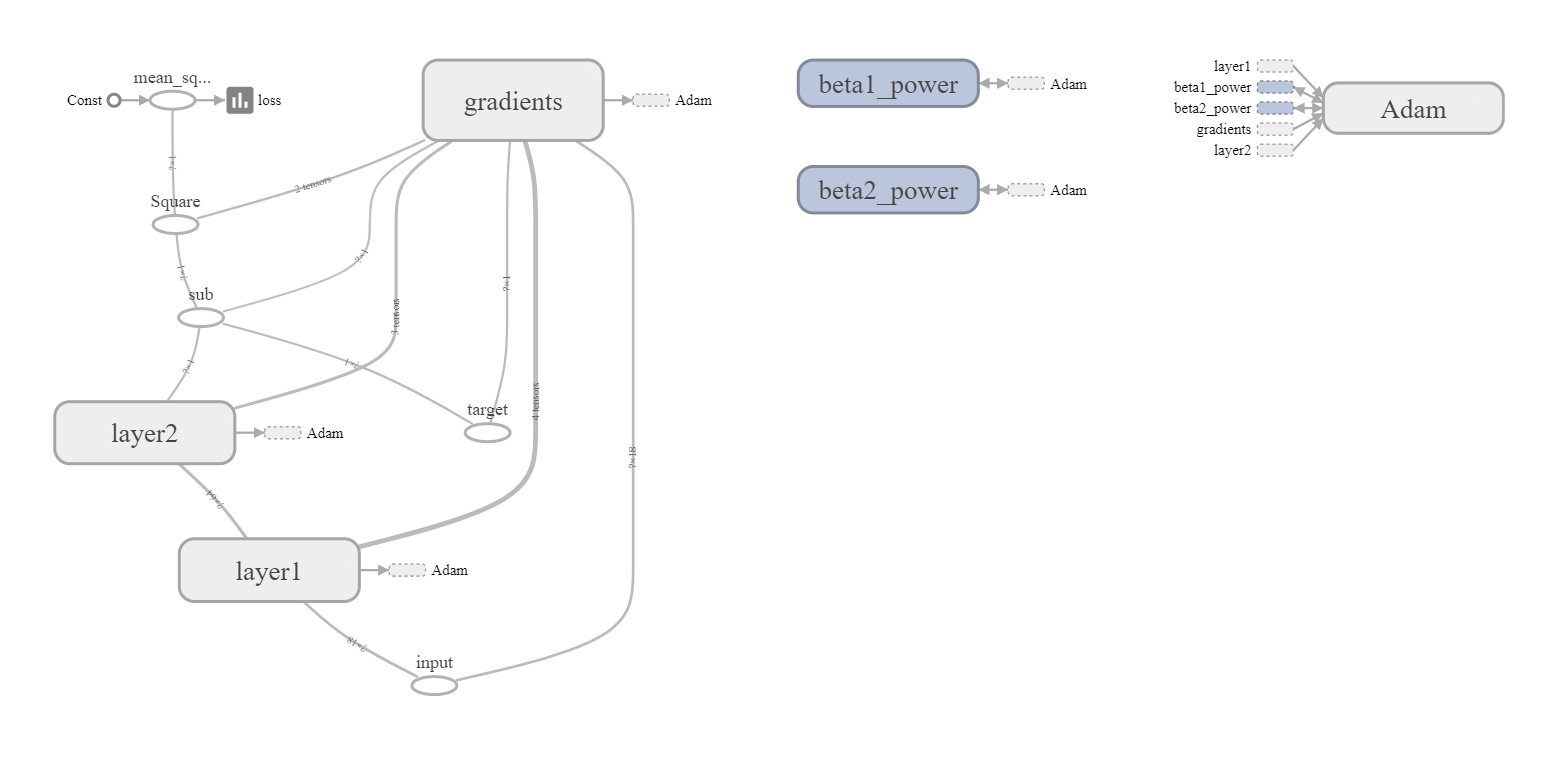
\includegraphics[width=13cm]{graph_relu_adam.png}